\ifx\wholebook\relax \else

\documentclass[UTF8]{article}

\input{../common-zh-cn.tex}

\setcounter{page}{1}

\begin{document}

\title{群、环、域}

\author{刘新宇
\thanks{{\bfseries 刘新宇} \newline
  Email: liuxinyu95@gmail.com \newline}
  }

\maketitle
\fi

\markboth{群、环、域}{编程的数学原理}

\ifx\wholebook\relax
\chapter{群、环、域}
\numberwithin{Exercise}{chapter}
\fi

\epigraph{你只要能把自己提出的那些“点、线、面”都说的跟“桌子、椅子、啤酒杯子”一样自然连贯就行。}{——大卫$\cdot$希尔伯特}

\begin{wrapfigure}{R}{0.3\textwidth}
 \centering
 \includegraphics[scale=0.35]{img/Escher-Liberation-1955.eps}
 \captionsetup{labelformat=empty}
 \caption{艾舍尔《解放》}
 \label{fig:clay-token}
\end{wrapfigure}

我们人类在长期的生产生活中逐渐养成了对事物分类整理的习惯。不同但相近的东西被归为一类。对整个类适用的性质和方法,对类中的不同事物都有效。这样我们就从解决具体的单一的问题,提高到一下子解决整类的抽象的问题,极大地丰富了我们认识掌握世界的能力。

在第一章中,我们曾经从自然数的累加和阶乘中归纳抽象出了“叠加”操作。我们观察它们相似的结构,将累加中的0和阶乘中的1抽象成单位元,将累加中的加法和阶乘中的乘法抽象成某种二元运算,这样就在更高的层次抽象出了自然数的叠加。进而可以用这一抽象的叠加操作解决诸如斐波那契数列这样的一大类和自然数同构的问题。

再举一个例子。我们在第一章中,还定义了列表上的抽象叠加操作$foldr$。可以利用这个抽象工具把一列数累加起来:$sum = foldr(0, +)$,也可以把一列数乘到一起:$product = foldr(1, \times)$。在计算机程序中,人们可以定义一种叫做“二叉搜索树”的数据结构。第二章中,我们曾经介绍过二叉树的定义。二叉搜索树是一种特殊的二叉树,它要求树中元素的类型A是可以比较的\footnote{这里比较的含义是抽象的,例如可以比大小,也可以是比较单词在字典中的先后顺序},并且对于任意分支节点,节点左侧子树中的所有元素都在此节点的元素之前,而右子树中的所有元素都在此元素之后。对排序二叉树,我们可以定义一个插入操作:

\[
\begin{array}{rcl}
  insert(nil, x) & = & node(nil, x, nil) \\
  insert(node(l, y, r), x) & = & \left.
  \begin{cases}
  x < y\ : & node(insert(l, x), y, r) \\
  x > y\ : & node(l, y, insert(r, x))
  \end{cases} \right.
\end{array}
\label{eq:BST-insert}
\]

根据这一定义,将一个元素$x$插入到二叉搜索树时,如果树为空,则结果为一个$node(nil, x, nil)$;否则,需要进一步比较$x$和分支节点中的元素$y$,如果$x$在前(用小于号代表),则递归地插入到左子树,否则地归地插入到右子树。联想累加和阶乘,插入操作和它们有什么相似之处呢?插入也是一个二元操作,而nil相当于单位元。这样我们就可以用抽象的叠加操作,将一列数字变成一棵搜索树:

\[
build = foldr(nil, insert)
\]

图\ref{fig:bst-example}展示了计算$build\ [4, 3, 1, 8, 2, 16, 10, 7, 14, 9]$产生的一棵二叉搜索树。

\begin{figure}[htbp]
  \centering
  \includegraphics[scale=0.5]{img/bst-example.ps}
  \caption{通过叠加产生的二叉搜索树}
  \label{fig:bst-example}
\end{figure}

我们人类对加法的认识也经历了类似的过程,最初的加法是针对具体事物的,例如采集的果实或者猎物。然后逐渐将具体事物的意义去除变成了针对抽象整数的加法。后来对数的认识扩充到了分数,虽然分数的具体相加过程和整数大相径庭,需要先进行通分,然后再将分子按照整数的法则相加,最后再进行约分。但是我们进一步将这两种不同的操作抽象成了有理数上的加法,人们深入思考它们的本质和性质,在每一次扩充数的认识时,都重新定义更加抽象的加法。从而有了实数上,复数上的加法。

\section{群}

\section{环}

\section{域}

\ifx\wholebook\relax \else
\begin{thebibliography}{99}

\bibitem{HanXueTao16}
韩雪涛 ``数学悖论与三次数学危机''. 人民邮电出版社. 2016, ISBN: 9787115430434

\end{thebibliography}

\expandafter\enddocument
%\end{document}

\fi
